 %	Skriv folgende ind som en custom Quick Build (F1)
%pdflatex -interaction=nonstopmode %.tex|bibtex %|pdflatex -interaction=nonstopmode %.tex|pdflatex -interaction=nonstopmode %.tex

\documentclass[english,twoside,openright]{report}

\usepackage[latin1,ansinew]{inputenc}
\usepackage[T1]{fontenc} 
\usepackage{babel}

\usepackage{rotating}
\usepackage[ansinew]{inputenc}
\usepackage{graphicx}
\usepackage{wrapfig}
\usepackage{float}
\usepackage{lipsum}
\usepackage{lastpage}
\usepackage{fancyhdr}
\usepackage{hyperref}    % Creates links in the PDF
\usepackage{listings}
\usepackage{algorithmic}
\usepackage{listings}
\usepackage{subfig} %til resize af billeder
\usepackage[usenames,dvipsnames]{color}
\definecolor{lightgray}{RGB}{232,232,232}
\usepackage{spverbatim} %Bruges til at indføre wrapping i kodemiljøer, ellers er den magen til {verbatim}

\lstdefinelanguage{cs}
  {morekeywords={abstract,event,new,struct,as,explicit,null,switch
		base,extern,object,this,bool,false,operator,throw,
		break,finally,out,true,byte,fixed,override,try,
		case,float,params,typeof,catch,for,private,uint,
		char,foreach,protected,ulong,checked,goto,public,unchecked,
		class,if,readonly,unsafe,const,implicit,ref,ushort,
		continue,in,return,using,decimal,int,sbyte,virtual,
		default,interface,sealed,volatile,delegate,internal,short,void,
		do,is,sizeof,while,double,lock,stackalloc,
		else,long,static,enum,namespace,string,MySQLTools,MySqlDataAdapter },
	  sensitive=false,
	  morecomment=[l]{//},
	  morecomment=[s]{/*}{*/},
	  morestring=[b]",
}

\lstdefinelanguage{nisse}
     {morekeywords={@begin,@end,@setting,fade,slide},
	  sensitive=false,
	  morecomment=[l]{//},
	  morecomment=[s]{/*}{*/},
	  morestring=[b]",
}


% CODE %
\usepackage{listings}
\usepackage{color}
\usepackage{textcomp}
\definecolor{listinggray}{gray}{0.9}
\definecolor{lbcolor}{rgb}{0.9,0.9,0.9}
\lstset{
	language=nisse,
	keywordstyle=\bfseries\ttfamily\color[rgb]{0,0,1},
	identifierstyle=\ttfamily,
	commentstyle=\color[rgb]{0.133,0.545,0.133},
	stringstyle=\ttfamily\color[rgb]{0.627,0.126,0.941},
	showstringspaces=false,
	basicstyle=\small,
	numberstyle=\footnotesize,
	numbers=left,
	stepnumber=1,
	numbersep=10pt,
	tabsize=2,
	breaklines=true,
	prebreak = \raisebox{0ex}[0ex][0ex]{\ensuremath{\hookleftarrow}},
	breakatwhitespace=false,
	aboveskip={1.5\baselineskip},
  	columns=fixed,
  	upquote=true,
 	extendedchars=true,
}


% URL %
\usepackage{url}
\makeatletter
\def\url@leostyle{\@ifundefined{selectfont}{\def\UrlFont{\sf}}{\def\UrlFont{\small\ttfamily}}}
\makeatother
\urlstyle{leo}


\setlength{\headheight}{15pt}
\pagestyle{fancy}
\renewcommand{\chaptermark}[1]{\markboth{#1}{}}
\renewcommand{\sectionmark}[1]{\markright{#1}{}}
 
 
\fancyhf{} % clear header and footer
\fancyhead[LO, RE]{\textit{\rightmark}}
\fancyhead[RO, LE]{\textit{\leftmark}}


\fancypagestyle{plain}{
\fancyhead[LE,RO,RE,LO]{}
\renewcommand{\headrulewidth}{0pt}
\fancyfoot[RO,LE]{\thepage\ of \pageref{LastPage}}}
\fancyfoot[RO,LE]{\thepage\ of \pageref{LastPage}}

\begin{document}
	
	\lstset{frameround=tttt, escapeinside={\%}{\%}}
	
	
	\title{Card Game Language}
\author{By: Group SW403F12}
\date{\emph{May 2012}}
\maketitle
\newpage
	\addtocounter{page}{1}
	\newpage
\addtocounter{page}{1}
\thispagestyle{empty}
\mbox{}
	\setcounter{page}{2}
	\thispagestyle{empty}
\begin{titlepage}
	\addcontentsline{toc}{chapter}{Titlepage}
	\setcounter{page}{3}
\begin{nopagebreak}
{\samepage 
\begin{tabular}{r}
\parbox{\textwidth}{  \raisebox{11mm}{
\includegraphics[height=1.2cm]{images/aau-logo.pdf}}
\hfill \parbox{4.9cm}{\begin{tabular}{l}
{\sf\small \textbf{Department of Computer Science}}\\
{\sf\small  \textbf{Aalborg University}} \\
{\sf\small Selma Lagerl\"{o}fs Vej 300} \\
{\sf\small Telephone: +45 9940 9940} \\
{\sf\small Telefax:   +45 9940 9798} \\
{\sf\small http://cs.aau.dk}
\end{tabular}}}
\\
\end{tabular}
\vspace{-12pt}
\begin{tabular}{cc}
\parbox{7cm}{
\begin{description}

\item {\bf Titel:} 

Airline Reservation System
  
\item {\bf Tema:} 

Developing applications from users to data, algorithms and tests and back again

\end{description}

\parbox{8cm}{

\begin{description}
\item {\bf Project period:}\\
   P3, Fall Term 2011\\
  \hspace{4cm}
\item {\bf Projectgroup:}\\
  SW306E11\\
  \hspace{4cm}
\item {\bf Partisipents:}\\
Jakob Lynge Albertsen\\
Johan S�rensen \\
Jonathen Bernstorff Nielsen\\
Tom Reinholdt Petersen\\
Tommy Knudsen
  \hspace{2cm}
\item {\bf Supervisor:}\\
Darius \v{S}idlauskas
\end{description}
}
\begin{description}
\item {\bf Circulation:} 7
\item {\bf Pagecount:} \pageref{LastPage}
\item {\bf Appendix count and type:} 6, Bibliography, Best-Path Algorithms, Protocol Specification, Process Analysis, Red Chair and a Danish Abstract.
\item {\bf Finished on} 19$^{th}$ Dec 2011
\end{description}
\vfill } &
\parbox{7cm}{
  \vspace{.15cm}
  \hfill 
  \begin{tabular}{l}
  {\bf Synopsis:}\bigskip \\
  \fbox{
    \parbox{6.5cm}{\bigskip
     {\vfill{\small This report describes...Synopsys
     \bigskip}}
     }}
   \end{tabular}}
\end{tabular}}
\\ \\
\noindent{\footnotesize\emph{The report content is freely available, but publication (with source), only after agreement with the authors.}}
\end{nopagebreak}
\end{titlepage}
	\chapter*{Signatures:}
	\addcontentsline{toc}{chapter}{Signatures}

\noindent\rule{8cm}{0.03cm}\\
Ali Mansour Nazim\\

\noindent\rule{8cm}{0.03cm}\\
Henrik Tudborg \\

\noindent\rule{8cm}{0.03cm}\\ 
Jakob Lynge Albertsen\\ 

\noindent\rule{8cm}{0.03cm}\\
Johan S�rensen\\

\noindent\rule{8cm}{0.03cm}\\
Jonathan Bernstorff Nielsen\\

\noindent\rule{8cm}{0.03cm}\\
Tommy Knudsen\\
	\tableofcontents	
	\addcontentsline{toc}{chapter}{Table of Contents}
	\newpage
	\chapter{Introduction}
Something something more general introduction to the report

\section{Server compiler}
A way to make the language more easy to compile is to take the workload off the user�s computer, and place it on a server. This creates the aspect that you can write and compile code anywhere, on any computer with internet, without any additional programs.
Having the compilation phase on a server, creates the possibility to write the program on a cellphone, which can send the code to the server and receive the presentation on the device.
With the internet getting faster and faster, more users are online, which doesn�t limit the users possibility when to compile. Altho the compiler can be downloaded for offline use if needed.
	\section{Problem statement}
Programming languages are often difficult and confusing for a beginner to understand. To this extent, there is no widespread language wherein card based games can be easily expressed and visualized.



%Mangler fortsat at blive rettet fra kortspil til slide shows!
	\chapter{Problem Formulation}
%The task of making a slideshow in applications like Microsoft�s Power Point or Apple�s Keynote is a mouse based task. How can you make a better alternative to \LaTeX~Beamer? How can you create a programming language in which a user can make a slideshow presentation without the need for a pointing device, and not have to think about the layout of single slides, but only define the general layout. Furthermore, how can you display the presentation in a way so that it will look equal on all computers. \\
%Challenges include creating a suitable domain specific language with weight on consistency and simplicity, enabling the user to focus on the content rather than the layout.

The task of making a slideshow in applications like Microsoft�s Power Point or Apple�s Keynote is a mouse based task. \\
How can you make a better alternative to \LaTeX~Beamer? \\
How can you create a programming language in which a user can make a slideshow presentation without the need for a pointing device, and not have to think about the layout of single slides, but only define the general layout? \\
Furthermore, how can you display the presentation in a way so that it will look equal on all devices? \\
A challenge regarding creating a suitable domain specific language with weight on consistency and simplicity is to enable the user to focus on the content rather than the layout.
\\ \\
The following questions provide a limitation for the scope of the project:
\\ \\
Which platform should be used for presentation? \\
Who are the users of the language? \\
Which layout decisions does the user need? \\
What are the language limitations? \\
What can be expressed in the language?
	
	% Part Analysis
	\part{Analysis}
	\chapter{Known Slideshow Applications}
In this section some of the best known applications, Microsoft PowerPoint, Apple Keynote and \LaTeX~Beamer, is compared to the solution developed during this project.
\\ \\
Microsoft PowerPoint and Apple Keynote are slideshows application which uses drag-and-drop functions, why they will not be focused more on, because this approach to create slideshows does not fullfill the requirements of being a non-pointing device based application, specified in the problem statement of this report. Because these violate the problem statement, the main focus will be on the differences between \LaTeX~Beamer and the slideshow programming language developed in this project.


\section{Beamer}

An example of \LaTeX~Beamer is as follows:

\begin{lstlisting}[frame=single, caption={Beamer example}, label=lst_beamer]
%\textbf{Main\_document.tex}%
\begin{document}

\include{Slide_document.tex}

\end{document}

%\textbf{Slide\_document.tex}%
\frame {
	\frametitle{Welcome to this course}

\textit{\fontfamily{uarial}\selectfont {This course will contain information about how you \underline{underline} things, and how you do other \textit{weight stuff} on sentences.} \\
\textbf{\fontfamily{uarial}\selectfont {Like this}} \\	}
}

%\begin{figure}[H]
	\centering
		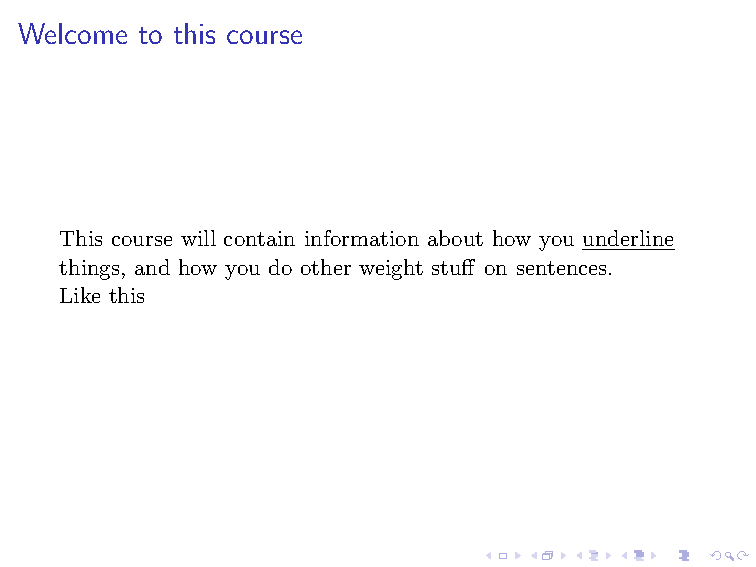
\includegraphics[width=0.8\textwidth]{text/beamer_example.pdf}
	\caption{\LaTeX~Beamer output}
	\label{fig:beamer_example}
\end{figure}%

\end{lstlisting}

The example seen in listing \ref{lst_beamer}, is the Beamer-code for expressing the output. The Beamer-code seen here is only to express output. To make a slideshow using Beamer you have to set up a main document. In this document, all the settings about what theme, colours, inputs (other files), etc., for the slideshow is set up. The editor (TexMaker) only generates a very small amount of the main document, which leaves a lot of setup for the user, if additional settings is wanted. If only a general slideshow is required, the main document will not need much work. A general slideshow is without colours, themes or the need for additional packages.\\
Compared to the Beamer-code the developed language should be made more compact to make slides faster to express.
\\ \\
A test between \LaTeX~Beamer and the developed language will be made to determine which and why one language is better than the other.
	\part{Analysis}
\chapter{Language Design}

This section has been based on the book ``Concepts of Progamming Languages'' \cite{CoPL}. The design of the language has been made using the language criteria in the table below. These criteria can be categorised into three primary categories; \textit{readability}, \textit{writability} and \textit{reliability}. These overall categories have a number of secondary categories, which will be used for specifying the language design. Which secondary categories that affects the overall categories can be seen in the table beneath.

\begin{table}[htbp]
\centering
\begin{tabular}{|l|c|c|c|c|}
\hline
\multicolumn{1}{|c|}{\textit{Characteristics}} & \multicolumn{3}{|c|}{\textit{Criteria}} \\ \hline
 & Readability & Writability & Reliability \\ \hline
Simplicity & X & X & X \\ \hline
Orthogonality & X & X & X \\ \hline
Data types & X & X & X \\ \hline
Syntax design & X & X & X  \\ \hline
Support for abstraction & & X & X  \\ \hline
Expressivity & & X & X \\ \hline
Type checking & & & X \\ \hline
Exception handling & & & X \\ \hline
Restricted aliasing & & & X \\ \hline
\end{tabular}
\caption{Language evaluation criteria from the book ``Concepts of Programming Languages''\cite{CoPL}}
\label{tbl:evaluation criteria}
\end{table}

\noindent{\textbf{Readability}} \\
Readability is one of the most important criteria in designing a programming language. The definition of readability is, that the language which is being designed should be easy to read and understand. When a programmer is adapting to a new language, the most difficult things to remember is usually the context of the language and the name of the data types. Creating a syntax, that in some way is similar to popular languages such as Java or C, would make the language more readable and easy to understand. \\
Readability of our programming language has been deemed ``less important'', because it is not as important as the writability or reliability, though it still has to be possible to read codes written in the language.
\\ \\
\textbf{Writability} \\
Writability is another important criteria in designing a programming language. It refers to how easy it is to write programs using the language, in this programming language it should be easy to write and express slides in the developed language. A programming language is usually easier to use, if it shares some characteristics with popular languages. However, a high writability ranking can also come from the language being simple to use. The writability has been deemed ``very important'', because our language is a slide show programming language, and considering that a slideshow is only made once.
%otherwise there is no reason for the programmer to learn a new language to express slide shows in.
\\ \\
\textbf{Reliability} \\
Reliability and correctness refers to how reliable a programming language is. The language is reliable if it performs correctly and without errors under all conditions, in this programming language meaning that the presentation behaves exactly as the user wants it to. The ability for the language to perform correctly under all conditions, has been deemed ``important'', because the user should be able to reli on the language in a way that makes them know what it would do, using the language.
\\ \\
\textbf{Cost} \\
When talking about the cost of making a programming language, there are some different aspects to consider, these are:
\begin{enumerate}
	\item The cost of training the programmers that is going to use the language, which is a function of simplicity, orthogonality and the experience of the programmers.
	\item The cost of writing programs in the language, which is a function of writability.
	\item The cost of compiling programs in the language.
	\item The cost of executing programs written in the language. In this part of performance the expression optimization is introduced, which is introduced to in-/decrease the size and/or the execution speed of the produced code. The reason that it can in- or decreased is that; programming beginners are compiling their programs frequently, whereas more experienced programmers are, potentially, executing their programs many times after the development of a certain program.
	\item The cost of implementing the programming language.
	\item The cost of, potential, poor reliability. If, for example, a system is unreliable, it can be costly to make it more reliable.
	\item The cost of maintaining programs written in the language, including corrections, modifications and additions to the program in question. Because maintenance is often done by other people than the original programmer, readability is of great importance, to ease the job of maintenance.
\end{enumerate}

\noindent{In the programming language of this project, the cost has been deemed ``less important'' because;}
\begin{itemize}
	\item It is not going to be taught to other programmers than the developers, because it is a proof of concept.
	\item The only programs that are going to be written in the language are written by the developers themselves.
%	\item As with writing programs in the language, the only programs that are going to be compiled in the language are the programs written by the developers themselves.
	\item As with writing and compiling programs in the language, the only programs that are going to be executed in the language are the programs written and compiled by the developers themselves.
  \item The language is not not ment to be developed for bigger cooporations, which is why the implementation of the language is held to a minimum.
%	\item The programs in the system will not be implemented in a bigger system, as to why the implementation costs are held at a minimum.
	\item The reliability is not that big a concern for this programming language, because the programs written herein will not be implemented as part of a greater system, as mentioned before, but it should be seen as a proof of concept.
	\item The maintenance will be kept as close to a minimum as possible, because when slideshows have been made, using the language, these will probably not be used again, which is why it will not be necessary to maintain them.
	\item The server, from which the code is being compiled, has to have some performance, because of the possibility of multiple programmers creating slides simultaneously. The performance is not the main focus, but it is important to make sure that there will not be unnecessary waiting for the programmers using the programming language. \\
\textbf{\textit{\underline{!!MAKE INTRUDUCTION TO (BEFORE) THIS SECTION!!}}}
\end{itemize}

\noindent{\textbf{Orthogonality}} \\
Orthogonality is the use of consistency, to avoid that some variable that has been assigned to a certain type, is being used another place assigned to another type.
\\ \\
\noindent{In the programming language of this project, the orthogonality has been deemed ``irrelevant'', because there are no types in the developed programming language.}
\\ \\
\textbf{Portability} \\
Portability is also known as the ease with which programs can be implemented on another platform than the one they were originally developed for. The way to make a programming language is by standardizing the language, which can be done by focusing on readability, reliability and writability, in particular. These do not standardize the language precisely, but provide a valuable insight into the design and evaluation of the programming language in question.
\\ \\
In the programming language of this project, the portability has been deemed ``very important'', because it is very important that the programming language is made in a way where it is working ``out of the box'', regardless of the operating system the programmer is using. Furthermore, the group who is to develop the programming language in question are using different operation systems, such as; Linux Ubuntu, Max OSx and Windows, which makes a good foundation for checking whether the programming language is working on these three operating systems, which gives the developers a good idea of the portability of the language. Furthermore, the slides created using the system should be able to be shown on different monitor/displays.
\\ \\
\textbf{Expressivity} \\
Is an expression covering the ease with which different operators in a programming language are designed. An example of this is using $count++$ instead of $count = count + 1$. Expressivity can
be seen as an extension to writability, in that it can make it easier to express statements in a programming. In the developed programming language, expressivity has been deemed ``important'' because there has been a lot of focus on making the language as easy and convenient to write and express slide shows in.
\\ \\
Beneath is a table with the language design criteria that has been designed for the programming language design for this project:
\begin{table}[htbp]
\centering
\begin{tabular}{|l|c|c|c|c|}
\hline
& Very important & Important & Less important & Irrelevant \\ \hline
Readability & & & X & \\ \hline
Writability & X & & & \\ \hline
Reliability & & X & & \\ \hline
Cost & & & X & \\ \hline
Orthogonality & & & & X \\ \hline
Portability & X & & & \\ \hline
Expressivity & & X & & \\ \hline
\end{tabular}
\caption{Language evaluation criteria defined for the programming language to be developed.}
\label{tbl:evaluation criteria}
\end{table}
	\section{Requirements}
The following requirements is set for the language to consider it as a complete language:

\textbf{Capabilities}\\
\begin{itemize}
\item The language has to make it possible to make bullet points and enumerations.
\item The language has to make it possible to import pictures from the Internet.
\item The user should be able to change font- type, color, size and line height.
\item The user should be able to make a transition between each slide. 
\end{itemize}
\textbf{Error handling}\\
\begin{itemize}
\item The language should be able to tell the user which line an error has occurred. 
\end{itemize}
\textbf{Test}\\
\item The language should be easy to write in, determined by the test:
\begin{itemize}
\item The experienced user of the language should be able to make five slides, with decent content, using standard settings, within 10 minutes, where the content is prewritten.
\end{itemize}
	\section{Types}
Type checking for the language is redundant, because no user made variables needs to be checked, because variables cannot be created by the user. The only variables in the language are the settings, which are set to either accept a number of chars or a number of digits. Mostly any other place consists of a number of chars.
	\section{Parser strategy}
Something med top-buttom, buttom-up parsing

	\chapter{Generating tool}

We use SableCC to generate the lexer and parser as it takes a modified version of EBNF as it's input. $\ldots$

\section{Output from tool}

Something Something output from tool
	
	% Part Solution
	\part{Solution}
	\part{Solution}
\section*{Introduction}
Constructing a compiler is split into four categories; lexer, parser, semantic analyser and code generator shown in \ref{fig:Compilerconstruction}.
The user inputs some code, the program he wants to be compiled, which is first met by the lexer. The lexer�s job is to make a token for each of the characters that is provided in the code. If a character is not recognized, this stage will fail.\\

%The token list is then given to the parser, which is building a parsetree, also called a Abstract syntax tree(AST), constructed from a context-free grammer. 

The parser asks the lexer for a token, which then is handled by the parser. This repeats itself until there are no tokens left. The parsers main function is to check the syntax of the source code, to check whether the source code contains any invalid sign of formatting. The parser is doing this by creating a parsetree, also called a Abstract syntax tree(AST), which it uses to check that all tokens are given in the right order. If the parser is able to create more then 1 AST, the code could behave differently each time it is compiled. There are also a number of ways for a parser to build an AST, which will be discussed later. If the parser fails to build a AST, this stage will fail.\\

The abstract syntax tree is then given to the semantic analyser...Something Something



\begin{figure}[! h]
\centering
	 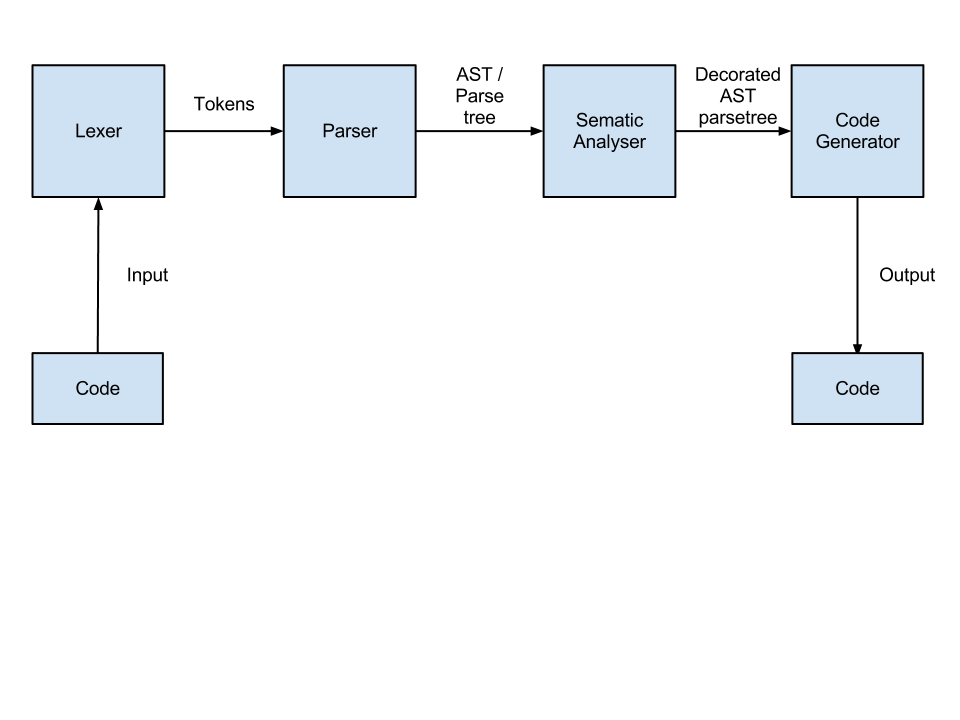
\includegraphics[width=250px]{images/Compilerconstruction.png}
		 \caption{Compiler construction}
	\label{fig:Compilerconstruction}
\end{figure}
	\chapter{Syntax}
\label{SSyntax}
The following example are some of the basic elements in the language:
\begin{verbatim}
Input:
@begin{fade|slide}
    Hello World
@end{|slide}
\end{verbatim}

\noindent{Output: Hello World}
\\ \\
Which states that a slide begins, with a transition ``fade'', and that the slide contains the text ``Hello World'' \\
The examples in the rest of this section is all written between @begin\{|slide\} and a @end\{|slide\} to save space.
\\ \\
After an @, a keyword always begins, making it easy for the compiler to recognize a keyword.
Here is another keyword ``Setting'', in this example the setting is set for the type ``title'' to a font size of 40 points. \\
A setting can be initiated outside, as well as inside, a slide. The difference is that, outside a slide the setting is applied to all the upcoming slides, if the setting is inside the slide, it is only applied to that slide. If no settings is set while making the slides, standard settings will be used.

\begin{verbatim}
Input: @setting{@font_size:40|title}
\end{verbatim}

\noindent{Output: (title font size set to 40)} \\

A way to use the title type can be by the following example:\\

\begin{verbatim}
Input: @title{|Hello and welcome}
\end{verbatim}

\noindent{Output: Hello and welcome (in the title format)}\\

As you see, there are nothing on the left side of the pipe (The sign before ``Hello''). Between the left curly and the pipe, settings can be applied to that specific sentence, like:\\

\begin{verbatim}
Input: @title{@font_size:70 |Hello and welcome}
\end{verbatim}

\noindent{Output: Hello and welcome (in title format with size 70)} \\


Which sets only this line of type ``title'' to font size 70, instead of 40 which was initialized above.
This can also be applied to normal sentences like:\\

\begin{verbatim}
Input: @apply{@font_size:25 | Welcome to this slide}
\end{verbatim}

\noindent{Output: Welcome to this slide (with font size 25)} \\

You have to use the keyword ``apply'', to change the format of a regular text. More than one format change can be applied pr. sentence, each format change does not necessarily need to be separated by one or more spaces. The order of format changes is irrelevant to the compiler. Here the font size is set to 25, and the text is ``Welcome to this slide''.

The weight of text can be done in two ways, the first looks like the way we just changed the font size:\\

\begin{verbatim}
Input: @apply{@font_weight:bold @font_size:25 | Welcome to bold text}
\end{verbatim}

\noindent{Output: \textbf{Welcome to bold text} (with font size 25)} \\

A quicker way to set a bold text is as follows:\\

\begin{verbatim}
Input: @b{|Welcome to bold text}
\end{verbatim}

\noindent{Output: \textbf{Welcome to bold text}} \\

Furthermore, we now want to underline a single word in that sentence:\\

\begin{verbatim}
Input: @b{|Welcome to @u{|bold} text}
\end{verbatim}

\noindent{Output: \textbf{Welcome to \textit{bold} text}} \\

Which make the whole text bold and underlines the word ``bold''.\\

Combining them, would look like this:\\

\begin{verbatim}
Input: @apply{@font_weight:bold | Welcome to @u{|bold} text}
\end{verbatim}

\noindent{Output: \textbf{Welcome to \textit{bold} text}} \\

And gives the same result as the last one. (eg. ref)

\subsection*{To summarize}
``@begin'' to start a slide\\
``@end'' to end a slide\\
``@b'' makes bold text \\
``@u'' makes underlined text \\
``@i'' makes italic text \\
``@apply'' changes a parameter for that line only\\
``@setting'' changes a parameter for the slide or globally.\\

The following is a larger example to demonstrate what is just used:\\

\begin{spverbatim}
Input:
@begin{fade|slide}
    @title{|@b{|Welcome to this course}}
    @setting{@font_type: Arial | text}
    This course will contain information about how you @u{|underline} things, and how you do other    
    @i{|weight stuff} on sentences.
    @apply{@font_weight:bold | Like this.}
@end{|slide}
\end{spverbatim}

\noindent{Output:} \\
\textbf{Welcome to this course} (as title) \\
This course will contain information about how you \underline{underline} things, and how you do other \textit{weight stuff} on sentences. (with font type Arial) \\
\textbf{Like this.}  (with font type Arial)
\\ \\

Settings does not have to be set at all, if they are not set, the standard settings will be used.

\section{Lists}
There are two types of lists, a list consists of either bullets or numerations.
A bullet list is made by writing the following:\\

\begin{verbatim}
Input:
List of things to buy
* 2 x milk
* Bread
** Light
* BKI coffee
\end{verbatim}
 
\noindent{Output:} \\
List of things to buy
\begin{itemize}
\item 2 x milk
\item Bread
\begin{itemize}
\item Light
\end{itemize}
\item BKI coffee
\end{itemize}

Where a star symbolises a bullet, and two bullets symbolises a bullet inside a bullet.
Numeration is made by the following: \\
Between the \# or * and the text related to the sign, does not necessarily need to be separated by a space, the text can also contain spaces and numbers if needed.\\

\begin{verbatim}
Input:
Agenda
# Introduction
# Presentation
## Code examples
# Evaluation
\end{verbatim}

\noindent{Output:} \\
Agenda
\begin{enumerate}
\item Introduction
\item Presentation
\begin{enumerate}
\item Code examples
\end{enumerate}
\item Evaluation
\end{enumerate}

Where a \# symbolises a number that incrementing. By using two \# creates a sub numeration starting from one.

\section{Images}
Importing pictures from the web and only from the web, can be done using the following code example:

\begin{spverbatim}
Input: @image{@url: http://www.danwec.com/images/foto/thumbs3/aau_logo.jpg  | Aalborg University logo}
\end{spverbatim}

\noindent{Output:} 
\begin{figure}[! h]
\centering
	 
\includegraphics[width=100px]{images/aau_logo.jpg}
		 \caption{Aalborg University logo}	
	\label{fig:Imageimport}
\end{figure}

Where the url to the image is before the pipe and after the keyword ``@url:''. The text after the pipe is the image text.
	\chapter{Lexer}
In this chapter the requirements of the lexer of NISSE will be presented, along with a listing of the tokens of NISSE.
\section{Requirements}
Requirements of the lexer:
\begin{itemize}
		\item The lexer should be able to take any plain text file as input
		\item The lexer should be able to recognize the input and make tokens according to the token list of NISSE
		\item The lexer should be able to output meaningfull error messages when it can not match the input to any token
		\item The lexer should be able to output the tokens so that the parser can use them
\end{itemize}
\section{Tokenlist}
In order to create the syntax in chapter \ref{SSyntax}, tokens has to be identified for later use.
\\ \\
The tokens for the language is as follows:

\begin{lstlisting}[frame=single]
format_kwd  = '@u' | '@b' | '@i' | '@apply' ;
space       = [\s]+ ;
settingkwd  = '@setting' ;
beginkwd    = '@begin' ;
endkwd      = '@end' ;
atsign      = [@] ;
lcurly      = [{] ;
rcurly      = [}] ;
pipe        = [|] ;
fslash      = [/] ;
bslash      = [\] ;
colon       = [:] ;
scolon      = [;] ;
blist       = [*] ;
nlist       = [#] ;
percent     = [(Percent sign)] ;
eol         = [\n |\r\n] ;
char        = ? [a-zA-Z \_ .,]+ ? ;
digit       = ? [ 0-9 ]+ ? ;
\end{lstlisting}

\noindent{The abnormal in this token list is the \texttt{``settingkwd��}, \texttt{``begindkwd��} and \texttt{``endkwd��} (kwd is short for: keyword). These keywords are explicit, because they are the keywords that differs from other keywords.}
\\ \\
The reason each special keyword has it�s own token, is to easily see the difference between the special tokens and the normal ones, without the need to check that a given token in the syntax analyser it is the right token.
\\ \\
\texttt{``Char��} is used whenever characters needs to used in the code. Char is also used for plain text, which require it to have the symbols underscore, backlash, comma and period. \\
\texttt{``Digit��} is used whenever numbers need to be used in the code. \\
When numbers or characters are expected, then one such has to occur at least once.
	\chapter{Parser}

In this chapter the requirements of NISSE will be presented, along with the context free grammar(CFG) of NISSE.

Requirements of the NISSE parser:
\begin{itemize}
	\item The parser should be able to receive tokens from the lexer, which it can then convert into a parse tree.
	\item It should be able to report useful error messages, if the user has written something illegal according to the CFG of NISSE.
	\item The CFG should be LL(1) in order to speed up the compiler.
	\item The CFG should also not be ambiguous, so that we can make a parser for it. Because the CFG is LL(1) (as per the previous requirement) the CFG is also not ambiguous as per the definition of LL(1).
\end{itemize}

The following is the CFG of the NISSE in EBNF:

\begin{lstlisting}[frame=single]
SS            = {Blocks} ;
Blocks        = BeginBlock {Lines} EndBlock 
              | SettingBlock ;
Lines         = SettingBlock 
              | Numeration
              | Itemlist 
              | Plains eol ;
Numeration    = nlist (Plains eol | Numeration) ;
Itemlist      = blist (Plains eol  | Itemlist) ;
BeginBlock    = beginkwd BEBlock eol ;
EndBlock      = endkwd BEBlock eol+ ;
BEBlock       = lcurly [space] char [space] [pipe char [space]] rcurly ;
SettingBlock  = settingkwd lcurly ShortIdent [space] pipe [space] char [space] rcurly eol;
Plains        = (ShortBlock | CharAll)+ ;
ShortBlock    = format_kwd lcurly [space] [ShortIdents] Plains rcurly ;
ShortIdents   = {ShortIdent}+ pipe ;
ShortIdent    = Kwd [space] colon [space] (char | digit) [space] ;
Kwd           = atsign char ;
CharAll       = colon 
              | digit 
              | scolon 
              | percent 
              | fslash 
              | bslash 
              | char 
              | space ;
\end{lstlisting}

This grammar is able to construct everything that is required of NISSE. \\
Let's look at one of the previous examples:

\begin{lstlisting}[frame=single]
Input:
@begin{fade|slide}
    Hello World
@end{slide}
\end{lstlisting}

The parse tree for this would look like: 

\begin{figure}[! h]
\centering
	 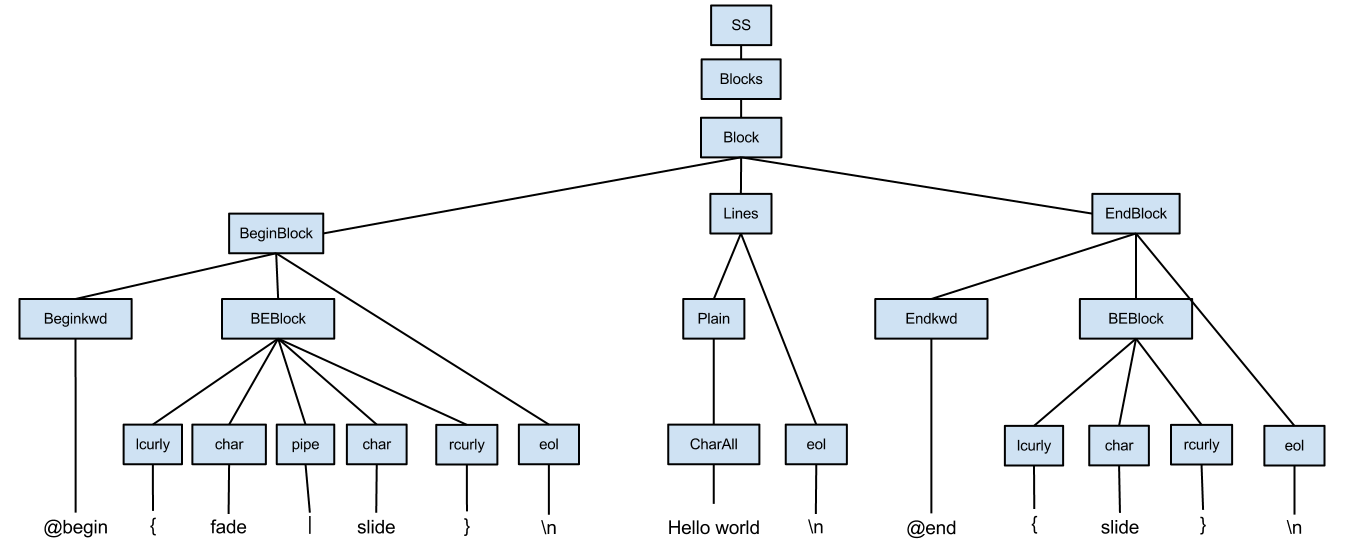
\includegraphics[width=300px]{images/ebnfexample.png}
		 \caption{Parsetree for a simple slide.}	
	\label{fig:Parsetree}
\end{figure}

%\begin{figure}[! h]
%\centering
%	 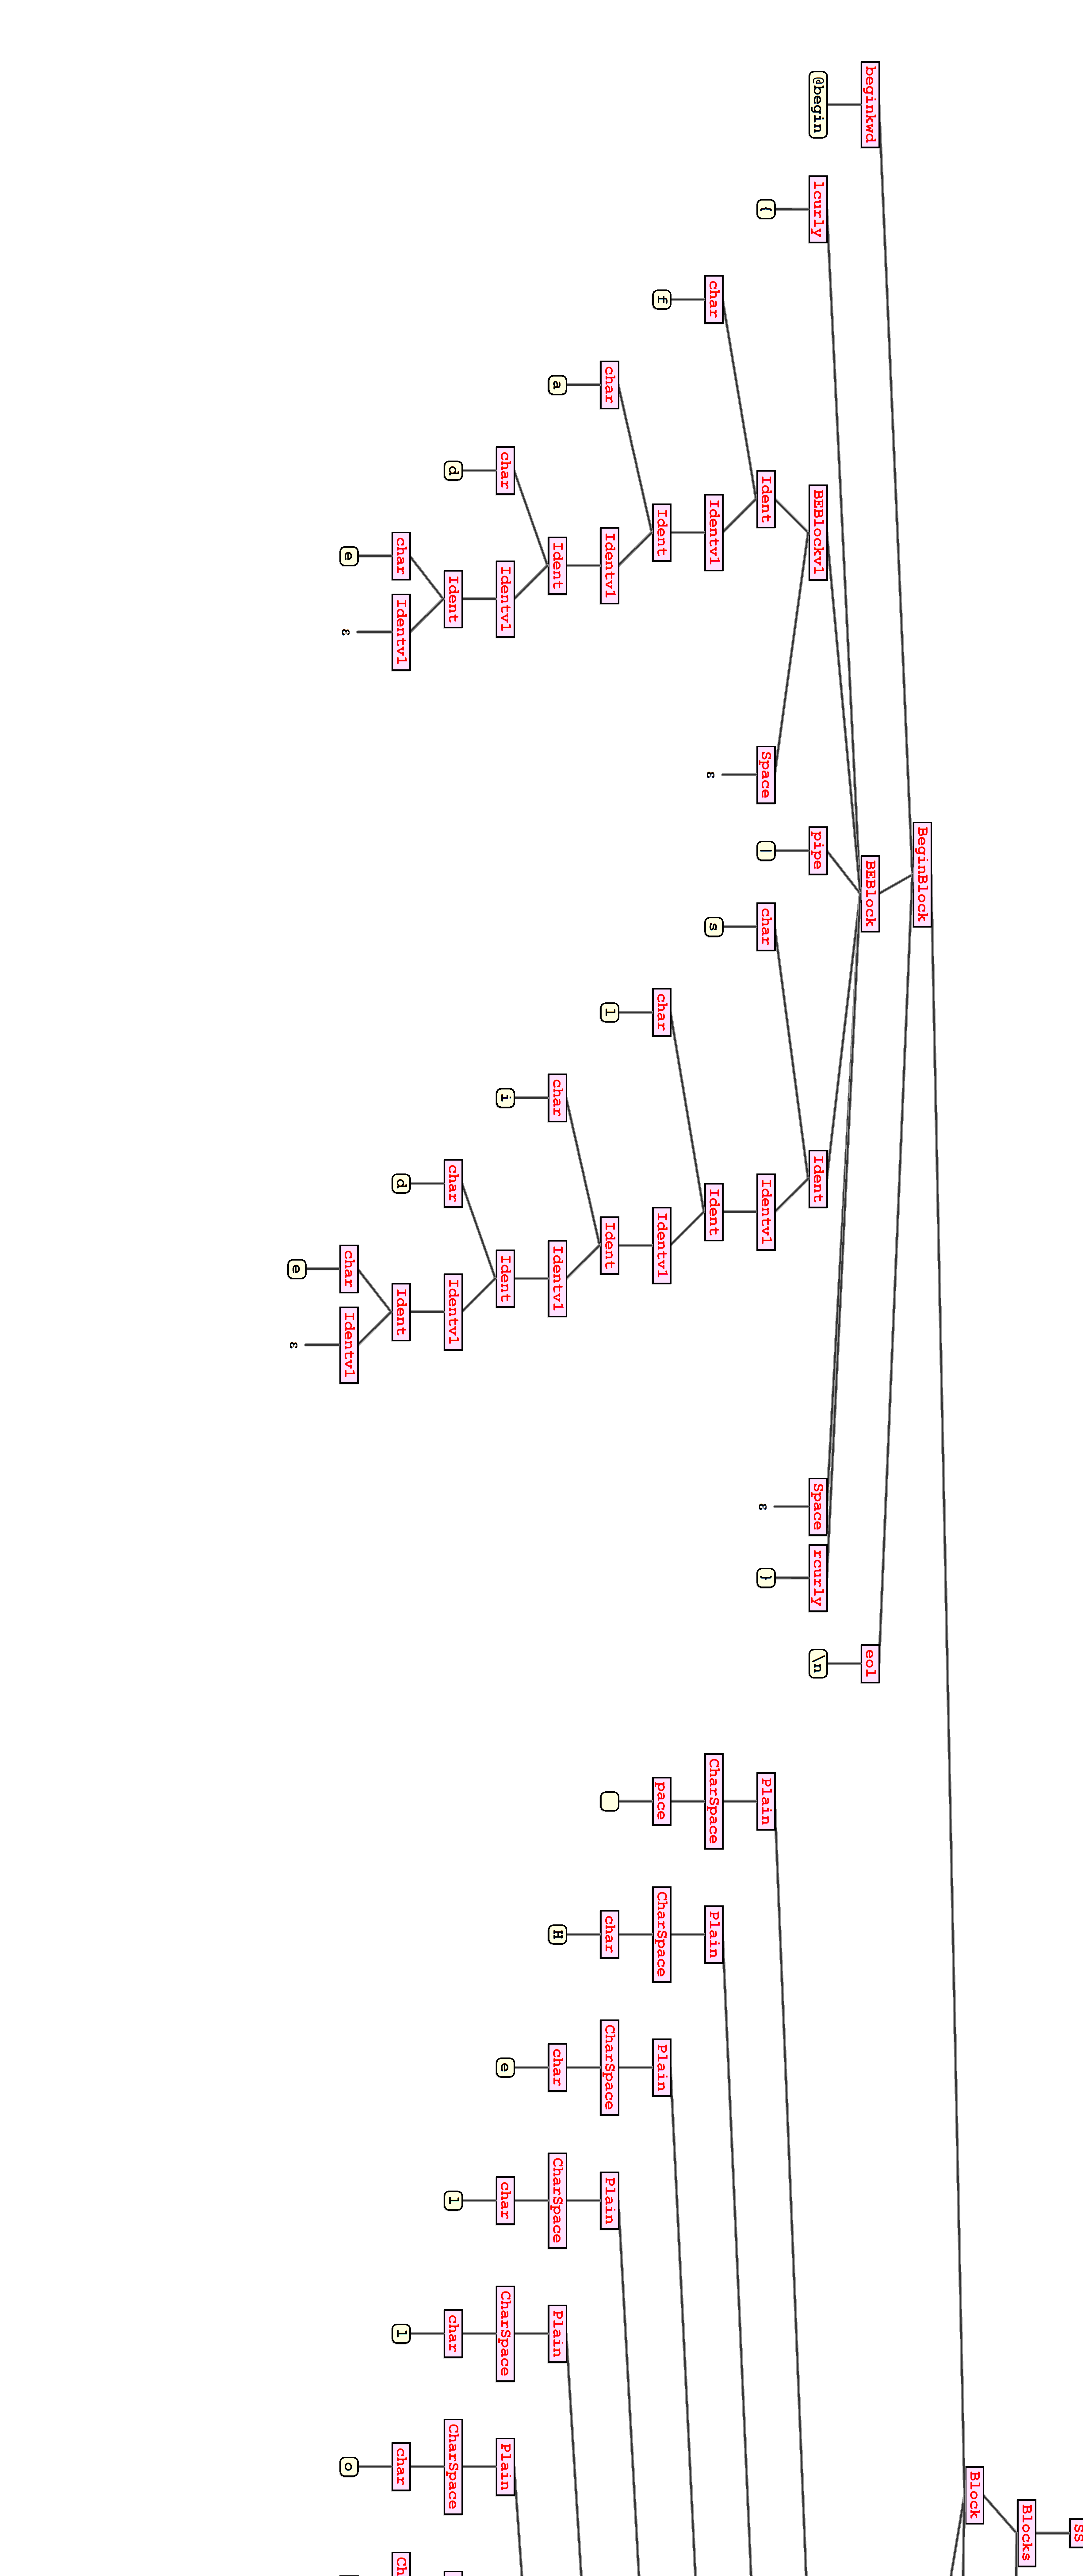
\includegraphics[width=270px]{images/Parsetreehalf(1).png}
%		 \caption{First half of parsetree for a simple slide. Using the program kfG}	
%	\label{fig:Parsetree}
%\end{figure}
%
%\begin{figure}[! h]
%\centering
%	 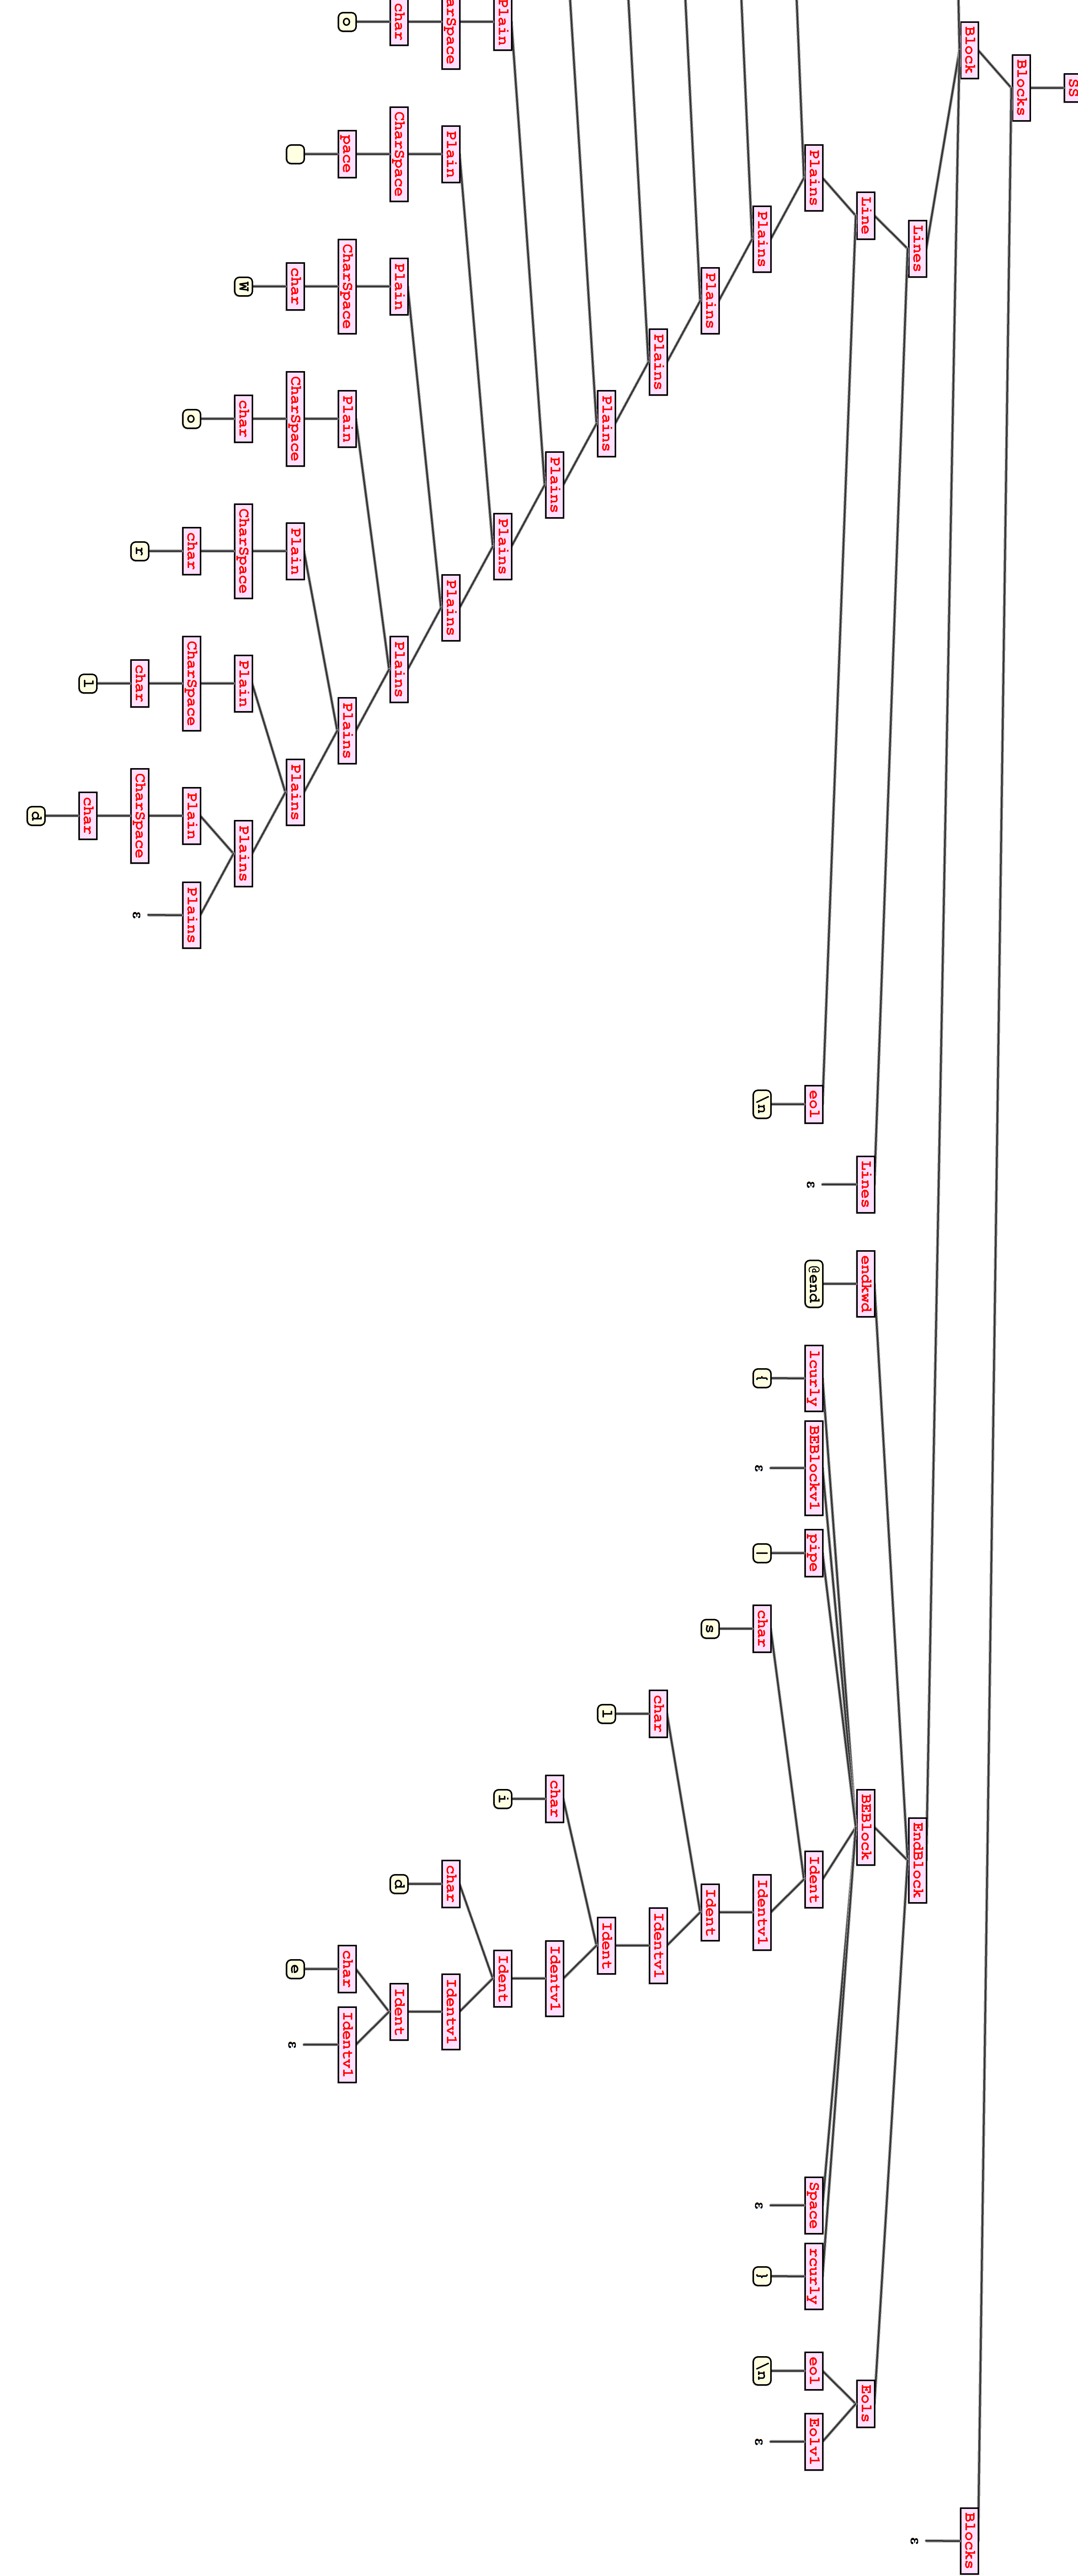
\includegraphics[width=270px]{images/Parsetreehalf(2).png}
%		 \caption{Second half of parsetree for a simple slide. Using the program kfG}	
%	\label{fig:Parsetree}
%\end{figure}

%The figure \ref{fig:Parsetree} is generated by the program ``kfG��, which has a slightly different structure, because each ``plain�� does not contain multiple characters. 
The figure \ref{fig:Parsetree} shows how it would parse the tree, with the input in a slide of �Hello World''. 
%The kfG structure can be seen in appendix \ref{AkfG}. We have chosen not to show anything that is more complex than the parse tree\ref{fig:Parsetree}, because the complexity would increase greatly.
	\chapter{Semantic analyser}

The semantic analyser checks for errors that the lexer and parser does not catch. The semantic analyser for the language has to have the following requirements for the code generator to be successful.

\section{Requirements}
\begin{itemize}
	\item Check that the dynamic keyword exists, in the language.
	\item Check that setting in the setting block exists.
	\item Check that it is a valid input after the colon in a setting block.
	\item Check that it is a valid scope on the right side of the pipe in a setting block.
	\item Check that the transition exists in a begin block.
	\item Check which number to put into the enumerate.
\end{itemize}

These requirements are put into categories, with more explanation to specify the function of the semantic analyser.

\section{Semantic analysis for text formatting}

    \subsection{Keyword existence}
In order for settings to work, a check to see if the given setting actually exists in that context is needed. In order to check if the setting exists, a list of settings for a given context is set up beforehand so that it can be checked against. If the setting exists in the list the value of the setting is checked to see if it matches a valid value of that setting. If it does not exist then an error is written to the user.

    \subsection{Type checking}
For a given setting there are a number of valid values, two examples could be the settings \texttt{font\_size} and \texttt{font\_weight} , which sets the size or weight of a given text. In the case of \texttt{font\_size}, valid input would be any integer, and in the case of \texttt{font\_weight} it would be a valid string of a weight. Same as the keyword existence an error is written if the value of the setting is not valid.

     
\subsection{Scope checking}

\subsubsection*{Targeted text}
Every setting block has to be given a scope of what it is going to affect. An example could be \texttt{global}, which, for a given setting would set all types of text in the given effect level unless it is overridden at a later stage.
\subsubsection*{Effect level}
When a setting block is inside a begin- and end block, the setting only affects that particular slide.
A setting block can also be used outside a slide, in which case that setting would apply to every slide following that setting unless overridden at a later stage. These scope settings has to be checked as to see what text that setting should apply to.

\section{Semantic analysis for blocks}
This section focus on blocks. A block consists of two lines, a \texttt{begin} line and an \texttt{end} line.
Between those two lines information can be stored.
The generic setup for the two lines is shown in section \ref{@begin} and \ref{@end}.

    \subsection{Transition existence}
In order for the compiler to apply a transition on a slide, the analyser has to check if the transition that is written exists in the database of transitions. If the transition does not exist an error has to occur. If the transition does exist, then it continues without error.

    \subsection{Type checking}
The type checking in a begin / end line, consists of checking that between the two brackets is the word texttt{slide}. In special cases, where a transition in on a slide, the word texttt{slide} must be between the pipe and the right bracket. The word seem redundant because no other word can be in its place at this time. But for further development, where a begin / end line can do more than just enclose a slide, this will come in hand.


\section{Semantic analysis for other keywords}
     \subsection{Image}
\texttt{Image} has to check if there exists an image on that specific url. If no image is found, accessible or in a format that is not recognized by the compiler, an error should occur.


     \subsection{Enumerate}
The hash tag keyword has to keep track of the numbers. Meaning that it has to increment each time a line starts with hashtag. And when a line does not start with a hash tag, the number should start from 1 again. This is also applicable where hash tags are inside hash tags.

\section{Exception handling}




\section{Reachability and termination analysis}
There are no need to check for unreachable code in the language, because there are no breakers in the language eg. return, break, exit, etc.
This also means that the language always terminates normal, because there are no keywords to stop a normal termination. 
	\chapter{Code Generator}

Something something much about Code generator
	
%	\input{text/parser/Parser}
	
	\part{Appendix}
	\appendix{}
	\chapter{Appendix}
\section{kfG}
\label{AkfG}
This is the settings used in the program kfG Edit, to be able to write AST examples of the defined language.
\begin{lstlisting}[frame=single]
SS           -> Blocks 
Blocks       -> Block Blocks | EPSILON 
Block        -> BeginBlock Lines EndBlock | SettingBlock
Lines        -> Line Lines | SettingBlock Lines | EPSILON 
Line         -> List | Plains eol
List         -> Numeration | Itemlist 
Numeration   -> nlist Numv1 
Numv1        -> Plains eol | Numeration 
Itemlist     -> blist Itemv1 
Itemv1       -> Plains eol | Itemlist 
BeginBlock   -> beginkwd BEBlock eol
EndBlock     -> endkwd BEBlock Eols
BEBlock      -> lcurly BEBlockv1 pipe Ident Space  rcurly
BEBlockv1    -> Ident Space | EPSILON
SettingBlock -> settingkwd lcurly Kwd colon Settingv1 Space pipe String rcurly eol
Settingv1    -> Ident| Number
Plains       -> Plain Plains | EPSILON
Plain        -> ShortBlock | CharSpace | Number
ShortBlock   -> Kwd lcurly ShortIdents pipe Plains rcurly
ShortIdents  -> ShortIdent | EPSILON 
ShortIdent   -> Kwd colon Settingv1 Space ShortIdents
String       -> CharSpace Stringv1
Stringv1     -> String  | EPSILON
CharSpace    -> char | pace
Ident        -> char Identv1
Identv1      -> Ident | EPSILON
Number       -> digit Numberv1
Numberv1     -> Number | EPSILON
Kwd          -> atsign Ident
Space        -> pace Space | EPSILON
CharAll      -> colon | char | digit | nlist | blist | scolon | percent | fslash | bslash
Eols         -> eol Eolv1
Eolv1        -> Eols | EPSILON



pace       -> ' ' 
settingkwd -> '@setting'
beginkwd   -> '@begin'
endkwd     -> '@end' 
atsign     -> @
lcurly     -> { 
rcurly     -> } 
seperator  -> <> 
pipe       -> '|' 
fslash     -> /
bslash     -> \
colon      -> : 
scolon     -> ; 
blist      -> * 
nlist      -> # 
percent    -> % 
eol        -> \\n | \\r\\n 
char       -> a|b|...|z|A|B|...|Z| \_ |.|,
digit      -> 0|1|...|9
\end{lstlisting}


\section{CFG(SableCC)}
\label{SableCC}
This is the settings used in the program kfG Edit, to be able to write AST examples of the defined language.
\begin{lstlisting}[frame=single]
charv1    = ['a' .. 'z'] | ['A' .. 'Z'] | '�' | '�' | '�' | '�' | '�' | '�' | '_';
digitv1   = ['0' .. '9'] ;
dot         = . ;
comma       = , ;
eolv1       = 13 10 | 13 | 10;
format_kwd  = @u | @b | @i | @apply | @image | @title | @subtitle | @note ;
url         = @url ;
space       =  ' ' ;
settingkwd  = @setting ;
beginkwd    = @begin ;
endkwd      = @end ;
atsign      = @ ;
lcurly      = { ;
rcurly      = } ;
pipe        = | ;
fslash      = / ;
bslash      = \ ;
colon       = : ;
scolon      = ; ;
blist       = * ;
nlist       = # ;
percent     = percent ;
exclamation = ! ;
eol         = eolv1+ ;
char        = charv1+ ;
digit       = digitv1+ ;
float       = digitv1+ dot digitv1+ ;
dot         = dot+;
comma       = comma+ ;
 
nisse         = blocks* ;
blocks        = {block} beginblock lines* endblock 
              | {setting} settingblock ;
lines         = {setting} settingblock 
              | {numeration} numeration
              | {itemlist} itemlist 
              | {plaintext} plains eol ;
numeration    = nlist numerationv1 ;
numerationv1  = {plaintext} plains eol 
              | {numeration} numeration;
itemlist      = blist itemlistv1 ;
itemlistv1    = {plaintext} plains eol  
              | {itemlist} itemlist;
beginblock    = beginkwd space* beblock eol ;
endblock      = endkwd space* beblock eol ;
beblock       = lcurly [first]:space* char [second]:space* beblockv1? rcurly ;
beblockv1     = pipe [first]:space* char [second]:space*;
settingblock  = settingkwd lcurly shortident pipe [second]:space* char [third]:space* rcurly space* eol;
plains        = plainsv1+;
plainsv1      = {shortblock} shortblock 
              | {charall} charall;
shortblock    = $format_kwd$ space* lcurly shortidents? plains rcurly ;
shortidents   = shortident+ pipe ;
shortident    = $kwd space*$ colon [first]:space* shortidentv1+ [second]:space*;
shortidentv1  = {char} char 
              | {digit} digit
              | {float} float
              | {colon} colon
              | {fslash} fslash
              | {dot} dot;
kwd           = {at} atsign char
              | {url} url ;
charall       = {colon} colon
              | {digit} digit
              | {semicolon} scolon
              | {percent} percent
              | {forwardslash} fslash
              | {backslash} bslash
              | {exclamation} exclamation
              | {dot} dot 
              | {comma} comma
              | {char} char
              | {space} space ;
\end{lstlisting}

	\bibliographystyle{plain}
	\bibliography{kilder}
	\addcontentsline{toc}{chapter}{Bibliography}
	\newpage
	\appendix
	\newpage
\addtocounter{page}{1}
\thispagestyle{empty}
\mbox{}

\end{document}
